\documentclass[../ace.tex]{subfiles}

\begin{document}
\section{Microarchitettura CPU}
\subsection{La CPU}
Rete logica combinatoria: rete priva di memoria, che dati ingressi da' delle uscite indipendentemente
dal tempo.
Rete sequenziale: rete che ha memoria, macchina a stati finiti, che dati degli ingressi fornisce
delle uscite dipendenti dallo stato in cui si trova.

Dal punto di vista funzionale possiamo vedere la CPU, come composta da due parti: il data path e
l'unità di controllo.
Il data path di cui componente fondamentale è l'ALU, è una rete logica che si occupa di eseguire le istruzioni, mentre
l'unita di controllo è una macchina a stati finiti che comanda il data path su quali istruzioni eseguire.
\\
Possiamo schematizzare l'unità di controllo come una macchina a stati finiti a tre stati: fetch, decode ed execute.

\subsection{Architettura di riferimento RISC}
Analizziamo adesso un esempio di architettura RISC.

Gli indirizzi di memoria sono riferiti ai byte. Le istruzioni occupano sempre e solo una parola a 32 bit.
Le istruzioni ed i dati si trovano sempre in indirizzi multipli di 4, per questo motivo il program counter
è incrementato di 4 ad ogni istruzione.
Avremo anche 32 registri di uso generale a 32bit. L'insieme dei registri è chiamato register file.

In generale l'esecuzione all'interno di un processore passa attraverso 5 fasi:
una prima fase chiamata Instruction Fetch (IF) dove il processore carica dalla memoria l'istruzione,
successivamente la decodifica nella fase (FT) e la esegue nella fase di execute (EX).
Dopodiché in alcuni casi si ha un accesso alla memoria nella fase di Memory (ME), ed infine
in alcuni casi ho una fase di write-back (WB), dove il risultato delle operazioni è riscritto
nei registri.

Tutte le istruzioni di questa ISA, come già detto hanno una lunghezza fissa di 32bit, ed appartengono a
3 categorie:
\begin{itemize}
    \item Un primo aritmetico logiche,
        Nei primi 6 bit opcode (codice operativo),
        seguiti da 5 che indicano il primo registro sorgente,
        altri 5 bit che indicano il secondo registro,
        5 che indicano il registro destinazione
        ed i rimanenti 11 fanno riferimento all'operazione specifica dell'ALU (somma, sottrazione, ...).
        \begin{lstlisting}
    add  r4,r2,r5
    \end{lstlisting}

    \item Un secondo formato utilizzato per accesso alla memoria e salti condizionati.
        I primi 6 bit di codice operativo,
        a seguire altri 5 ad indicare il primo registro
        ed altri 5 ad indicare il secondo registro (come nel primo caso)
        16 che indicano un offset o un dato.

        \begin{lstlisting}
    je  r2,r3,0045h
        \end{lstlisting}
    \item Un terzo ed ultimo caso utilizzato per i salti incondizionati.
        I primi 6 bit indicano sempre l'opcode ed i rimanenti indicano l'indirizzo di termine del
        salto.

        \begin{lstlisting}
    jmp 0045h
        \end{lstlisting}
\end{itemize}
In questa prima architettura assumiamo che non ci sia lo stack (zona di memoria organizzata a pila LIFO),
accessibile attraverso istruzioni apposite come \lstinline{push} e \lstinline{pop}.

Oltre a salto condizionato ed incondizionato esiste un terzo tipo di salto: la chiamata a funzione.
È un tipo di salto incondizionato particolare, dato che quando eseguito è necessario salvare il valore
del program counter per poter proseguire l'esecuzione una volta terminata la funzione.

Siccome non abbiamo uno stack, il program counter è salvato nell'indirizzo $R_{31}$
%27: ragionamento di funzionamento dell'ALU

Per selezionare le operazioni da far eseguire all'ALU è specificato un ingresso chiamato opalu, dove vengono
specificate le operazioni. Oltre all'uscita dell'operazione vengono tornati dei valori aggiuntivi come
il flag di zero (messo ad uno quando il risultato dell'ALU è zero), ed il flag di segno (messo ad 1 quando il
risultato è negativo).

\subsubsection{Load e Store}
%35
Load e store permettono rispettivamente lettura e scrittura in memoria.
Entrambe prendono in ingresso un registro base, uno destinazione ed un offset. Per accedere al dato l'offset viene sommato
al registro base ottenendo un nuovo indirizzo, il cui contenuto è salvato nel registro destinazione.
I dati vengono direttamente presi dal bus attraverso buffer 3-state, lettura e scrittura possono essere disabilitate con i segnali
$Mr$ (\textit{Memory Read}) e $Mw$ (\textit{Memory Write}),

\subsubsection{Register File}
Componente che ha come ingressi 5 bit che identificano il primo registro, 5bit per il secondo registro,
5bit per il registro destinazione, ed i rimanenti 32 per il dato in ingresso.
Le due porte in uscita riportano i dati letti rispettivamente dal registro sorgente 1 e 2.
%49

\subsection{CPU monociclo}
% TODO: aggiungere disegno CPU monociclo
In una CPU monociclo, tutte le istruzioni impiegano un solo ciclo di clock. È una struttura molto semplice, ma potenzialmente anche molto
lenta, dato che il tempo di esecuzione di ogni istruzione deve essere pari al tempo di esecuzione dell'istruzione più lenta.

Prendendo come esempio l'istruzione \lstinline{st R6,R1, 20},
\begin{itemize}
    \item in fase di fetch: recupero istruzione dalla memoria.
    \item fase di decode
    \item fase di execute: salva dato in memoria.
\end{itemize}

\def\tmono{T_\text{mono}}
\def\tmulti{T_\text{multi}}

Dato che in un unico ciclo di clock devo eseguire sia fetch che store, devo necessariamente avere due memorie separate.
È inevitabile l'uso di un'architettura di Harvard (pagina \pageref{sec:architettura_harvard}).
Oltre alla doppia memoria portata dall'architettura è necessario duplicare altre risorse, come ad esempio l'ALU, richiesta
per incrementare sia valore del program counter che per calcolare l'indirizzo di destinazione del dato.

Tra le varie operazioni richieste dall'ISA, il tempo di esecuzione maggiore è dovuto sicuramente alla \lstinline{load} (vedi
tabella \ref{tab:tempi_esecuzione_monociclo}),
che oltre alle fasi di fetch e decode richiede: calcoli dall'ALU, writeback ed accesso alla memoria.
Chiamato il suo tempo di esecuzione $\tmono$ ed $N$ il numero di istruzioni, il tempo di esecuzione del programma è $\tmono \cdot N$.

\begin{table}[t]
    \centering
    \begin{tabular}{|c|c|c|c|c|c|c|}
        \hline
    & Fetch  & Decode & ALU & Memory & Writeback & Totale \\
    \hline
        Aritm.   & 30 & 5 &  12 &        &         5 &      52\\
        Load     & 30 & 5 &  12 &     30 &         5 &      82\\
        Store    & 30 & 5 &  12 &     30 &           &      77\\
        jmp cond.& 30 & 5 &  12 &        &           &      47\\
        jmp      & 30 & 5 &     &        &           &      35\\
        jal/call & 30 & 5 &     &        &         5 &      40\\
        \hline
    \end{tabular}
    \caption{Esempio tempi di esecuzione in architettura monociclo}
    \label{tab:tempi_esecuzione_monociclo}
\end{table}

% Lezione 2.6
\subsection{CPU multiciclo}
Suddivide ogni stadio di esecuzione dell'istruzione in un ciclo di clock.
Il ragionamento alla base di questa architettura è che molte istruzioni hanno un tempo di istruzione notevolmente inferiore ad altre.
In altre parole, chiamata $\sum\tmulti$ il tempo di esecuzione di una singola istruzione il numero di istruzioni per cui
$\sum\tmulti > \tmono$ sarà inferiore al numero di istruzioni per cui $\sum\tmulti < \tmono$.
Ne consegue che l'architettura multiciclo è in media più veloce dell'architettura monociclo.

\begin{figure}[h]
    \centering
    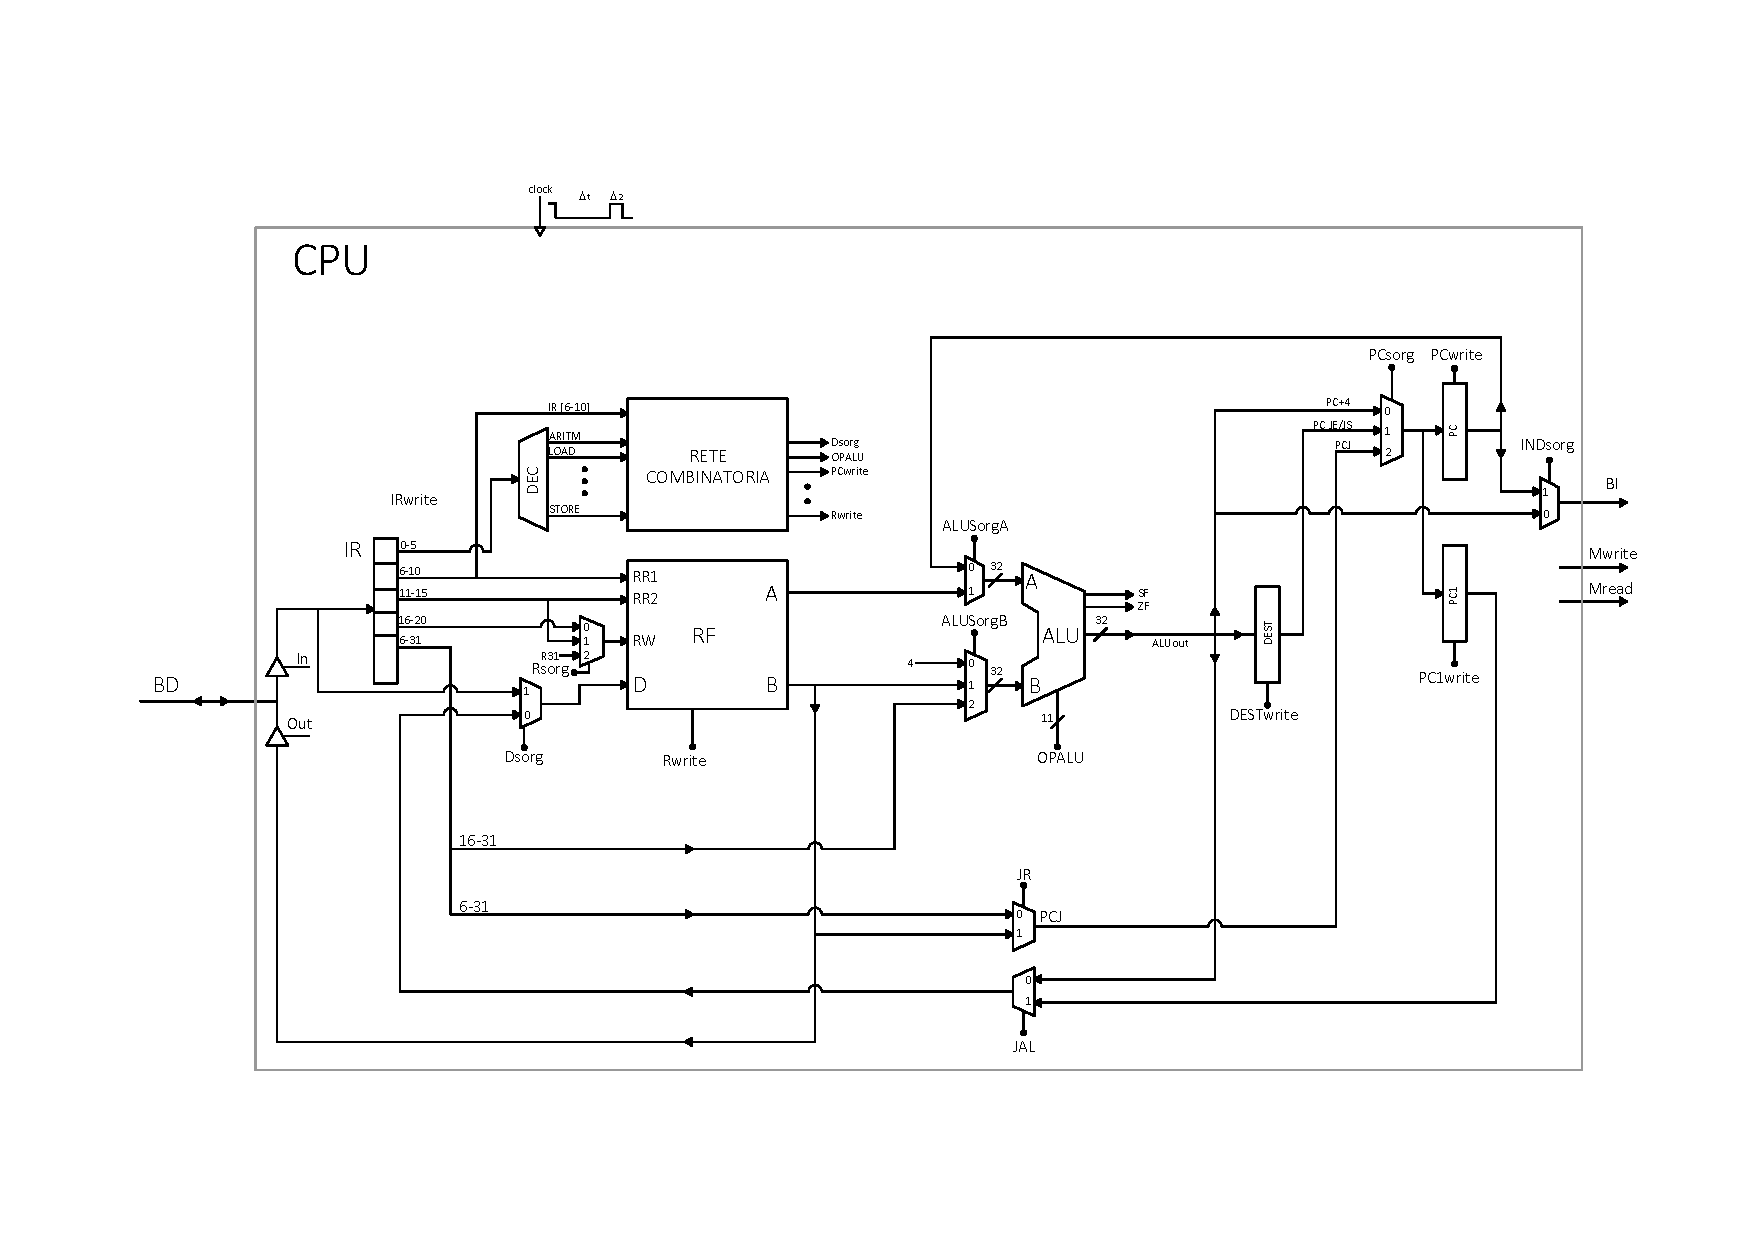
\includegraphics[width=\textwidth]{architettura_cpu}
\end{figure}
Non è più necessario duplicare componenti come ALU e memoria, dato che l'accesso ai dati e incremento PC/calcolo registri è
eseguito in due cicli di clock differenti.

% TODO: aggiungere schema generale architettura multiciclo (slide 60)
\begin{itemize}
    \item Fetch:
        Viene letto in memoria ll contenuto del program counter, e nello stesso ciclo attraverso l'alu aggiorno il program counter e lo
        salvo in pc.
    \item Decode:
        Analogamente alla precedente, il codice operativo di PC entra in IR, e viene decodificato.
        Leggo il contenuto dei registri R1 ed R2.
        Utilizzo l'alu per calcolare a prescindere il valore del registro di destinazione (destinazione del salto condizionato
        viene calcolata prima di verificare le condizioni)
    \item Operazione Aritmetica:
        Eseguo l'istruzione utilizzando i dati calcolati nelle fasi precedenti.
    \item Load e Store:
        Sempre attraverso buffer 3-state salvano o leggono dati dalla memoria all'indirizzo destinazione calcolato nelle fasi
        precedenti.
    \item Writeback:
        In caso di operazione aritmetica prendo il valore in uscita dell'ALU e lo riporto nel register file nella porta dati.
        In caso di load, il valore di uscita della memoria viene riportato nella porta dati del register file.
        In caso di JAL PC1 (valore precedente di PC) entra nel register file.
\end{itemize}

Interfacce con l'esterno: bus di dati attraverso buffer 3-state, in uscita al bus degli indirizzi arriva o alu-out o pc.


%2.7
\newcommand{\code}[1]{\oldlstinline[keywordstyle=\ttfamily]{#1}}

\subsubsection{Segnali di controllo architettura multiciclo}
La fase di instruction fetch, comune a tutte le istruzioni, richiede di leggere l'istruzione corrente dalla memoria ed
incrementare il program counter di 4. Per queste operazioni, sono necessari i segnali:
\begin{tabular}{ll}
    \code{M_r}& Memory Read\\
    \code{In} &abilitazione buffer 3state\\
    \code{PC_w}& program counter write\\
    \code{PC1_w}& program counter 1 write\\
    \code{IR_w} &instruction register write
\end{tabular}

Ed i seguenti segnali di selezione:

\begin{tabular}{ll}
    \code{INDsorg =1}& per scegliere di inviare alla memoria il valore del program counter\\
    \code{PCsorg=0} &per selezionare come ingresso di PC, PC+4\\
    \code{ALUsorgA = 0} &seleziona PC come ingresso A della ALU\\
    \code{ALUsorgB = 0} &seleziona 4 come ingresso B della ALU\\
    \code{OPALU =  ADD} &per eseguire una somma con la ALU
\end{tabular}

Nella fase di decode è richiesto di decodificare il codice operativo, inviare i due registri sorgente al register file
e sfrutto l'ALU non utilizzata per calcolare in anticipo l'indirizzo di destinazione gli eventuali salti condizionati.

Quindi è necessario il segnale \code{DESTw} per abilitare scrittura nel registro di destinazione, e i selettori
per l'ALU: \code{ALUsorgA=0}, \code{ALUsorgB=2} per indicare rispettivamente PC e l'offset come ingressi, e
\code{OPALU=ADD} per sommarli.

Passate queste due fasi, comuni a tutte le operazioni, vi è una differenziazione a seconda del tipo di istruzione
contenuta in \code{IR}.
In caso di istruzioni aritmetiche, composte da execute (T3) e writeback (T5), in prima fase, sono richiesti i segnali
per specificare le operazioni dell'alu (A = 1, B = 2, OP=ADD).
In T5 è richiesto \code{Rw} per scrivere nel registro destinazione contenuto in \code{RF}, e \code{Rsorg = 0}
\code{Rdest=0} per scrivere nel registro destinazione il alu-out.
L'istruzione passa anche attraverso una fase di memory (T4) ma vengono solamente mantenuti i valori in T3, tenere
costante il valore di alu-out.

Nella fase di execute di una load, viene calcolato l'indirizzo del dato in memoria \code{Rb + offset} (A=1, B=2, OP=ADD)
e salvato in \code{Rdest} .
In fase T4 \code{INDsorg = 0} e \code{Mr =1} per indicare di leggere il valore del dato all'indirizzo
di memoria calcolato dall'ALU.
In T5 viene salvato in \code{Rd} il dato letto dalla memoria \code{In=2} per mettere il bus dei dati in ingresso e
portare il segnale dalla memoria al processore, viene abilitato \code{Rwrite} per abilitare la scrittura al register file.
\code{Rsorg=1} e \code{Dsorg=1} per scrivere il registro \code{Rd} il dato proveniente dalla memoria.

In caso di store, i segnali nella fase di execute sono identici a quelli della load, ma eseguo \code{INDsorg=0} uno step
prima per avere il segnale stabile alla fase successiva e \code{Out=1}.
In T4 \code{Mw=1} per scrivere in memoria. Non ha una fase di writeback.

I salti condizionati richiedono solo un ciclo di completamento, in quanto l'indirizzo di destinazione è già stato
calcolato nella fase precedente, per resta solo da abilitare \code{PCw} in caso la condizione di salto sia verificata.
(A = 1, B=1, OP=SUB) \code{PCsorg=1} per selezionare \code{DEST} come ingresso a PC.

In caso di salti incondizionati esiste la sola fase T3 con \code{PCw=1} e \code{PCsorg=2}.

L'ultimo caso \lstinline{jal}, è del tutto identico ad un salto condizionato, solo che viene seguito da una fase di
writeback, in cui salvare \code{PC1} in \code{R31}.
\subsection{Prestazioni dell'architettura multiciclo}
\begin{wrapfigure}{R}{0pt}
    \centering
    \begin{tabu}{|l|lc|c|}
        \hline
        Aritm  & 5& 150ns &40\%\\
        \hline
        Load & 5& 150ns   &25\%\\
        \hline
        Store & 4& 120ns  &10\%\\
        \hline
        JE/JS& 3& 90ns    &12\%\\
        \hline
        JMP/JR& 3& 90ns   &6\%\\
        \hline
        JAL& 5& 150ns     &2\%\\
        \hline
    \end{tabu}
\end{wrapfigure}
Diversamente dall'architettura monociclo in cui $\tmono$ dipende dall'istruzione più lenta, il tempo $\tmulti$ dipende dallo
stadio più lento.
Prendendo come riferimento la tabella dei tempi di esecuzione dell'architettura monociclo (vedi pagina
\pageref{tab:tempi_esecuzione_monociclo}), ne consegue $\tmulti =30$
Confrontando quindi le varie fasi ottengo chiaramente che i tempi di esecuzione delle singole istruzioni, ed il tempo di
esecuzione medio è peggiore. Questo è dovuto ai $30ns$ della fase di fetch, che occupano più di 1/3 del tempo di
esecuzione di una singola istruzione.
\clearpage

\subsection{Miglioramenti architettura multiciclo}
L'architettura multiciclo per come vista sino ad ora è inefficiente, per migliorarla ci possono essere diversi modi:
\begin{itemize}
    \item Ridurre il periodo di clock, introducendo salti di attesa per le fasi più lunghe
    \item Sfruttare le componenti inutilizzate, calcolando in anticipo operazioni richieste in fasi successive
    \item Unire fasi distinte e modificare opportunamente il segnale di clock
\end{itemize}
\subsubsection{Aumento granularità del clock}
Avendo preso $\tmulti$ uguale al tempo d'accesso alla memoria, nelle fasi in cui essa è inutilizzata, c'è spreco di
tempo. L'ideale per questa architettura sarebbe che tutti gli stadi richiedano approssimativamente lo stesso tempo di
esecuzione.
Prendendo ad esempio $\tmulti=12$ (tempo dell'ALU), gli stadi di accesso alla memoria richiederanno 3 cicli di clock
($12\cdot 3 > 30$).

Svolgendo i calcoli otteniamo un tempo medio di $86.88ns$, migliore rispetto al precedente, ma ancora più lento rispetto
agli $82ns$ dell'architettura monociclo.

Osservando che con $\tmulti=12$ nelle fasi di memoria rimane uno spreco di $36-3\cdot 12=6ns$ riduciamo ancora la
granularità di clock a $\tmulti=5ns$ (fase più veloce: decodifica del writeback)
saranno richiesti quindi 6 cicli di clock per le fasi che fanno accesso alla memoria, e 3 per le fasi di ALU.
Il tempo medio per istruzione si riduce a $75.65ns$, migliore rispetto al caso precedente e dell'architettura monociclo.
\subsubsection{Anticipazione delle operazioni}
Partiamo dall'osservazione che in T2 si esegue un passo che serve solo a JE/JS. Possiamo quindi differenziare la fase T2
a seconda dell'istruzione. Inoltre, dato che il periodo è sufficientemente lungo, possiamo unire più istruzioni in un
unico ciclo di clock:

\begin{itemize}
    \item Per operazioni aritmetiche, dopo il fetch, richiedono una decodifica ed un operazione dell'ALU, con un totale
        di $5 + 12 + 5=22ns$ sufficiente da eseguirle nell'unica fase T2
    \item Per load il calcolo dell'indirizzo può essere fatto in T2, la lettura della memoria in T3 e scrittura nel
        registro destinazione in T4, tagliando un ciclo di clock.
    \item L'operazione di store, esattamente come per la load, anticipiamo il calcolo dell'indirizzo sorgente in T2,
        quindi la scrittura in memoria è effettuabile immediatamente all'istante T3.
    \item In JMP/JS è possibile aggiornare PC direttamente in T2
    \item In JAL è possibile aggiornare PC e la scrittura in R31. PC1 non è più necessario.
\end{itemize}

Il tempo di esecuzione medio è $81.60ns$, migliore della versione multiciclo originale e circa la stessa velocità
dell'architettura monociclo.

Aumentando la granularità di clock in quest'architettura, ipotizzando un $\tmulti=6 ns$ (dato che IF e ME richiedono
$6ns$), otteniamo un tempo medio di $64.76ns$ migliore del $21\%$ rispetto alla monociclo.

\end{document}
